\documentclass[11pt]{article}
\usepackage{amsmath, amssymb, amsthm, graphicx, geometry}
\usepackage{hyperref}
\geometry{margin=1in}

\title{CS461 Homework 5}
\author{Mannan Shukla}
\date{\today}

\begin{document}

\maketitle

\section*{Problem 1: Expectation-Maximization (EM) Algorithm}

\subsection*{1.1 Log-Likelihood Computation} The log-likelihood for the initial parameters is given by:
\[
\log L = \sum_{n=1}^N \log \left( \sum_{k=0}^1 \pi_k \cdot \mathcal{N}(x_n | \mu_k, \sigma_k^2) \right)
\]
where:
\[
\mathcal{N}(x_n | \mu_k, \sigma_k^2) = \frac{1}{\sqrt{2\pi \sigma_k^2}} \exp\left( -\frac{(x_n - \mu_k)^2}{2\sigma_k^2} \right)
\]
Using the initial parameters:
\[
\pi_0 = \pi_1 = 0.5, \quad \mu_0 = -1, \, \mu_1 = 1, \quad \sigma_0^2 = \sigma_1^2 = 1
\]
and the data points \( x = [2, 1, -1, -2] \), the initial log-likelihood is:
\[
\log L = -7.158.
\]

\subsection*{1.2 E-Step}
The responsibilities \( \gamma_{nk} \) are computed as:
\[
\gamma_{nk} = \frac{\pi_k \cdot \mathcal{N}(x_n | \mu_k, \sigma_k^2)}{\sum_{j=0}^1 \pi_j \cdot \mathcal{N}(x_n | \mu_j, \sigma_j^2)}.
\]
The resulting responsibilities are:
\[
\gamma =
\begin{bmatrix}
0.01799 & 0.98201 \\
0.11920 & 0.88080 \\
0.88080 & 0.11920 \\
0.98201 & 0.01799
\end{bmatrix}.
\]

\subsection*{1.3 M-Step}
The updated parameters are computed as follows:
\begin{align*}
\pi_k(t+1) &= \frac{1}{N} \sum_{n=1}^N \gamma_{nk}, \\
\mu_k(t+1) &= \frac{\sum_{n=1}^N \gamma_{nk} \cdot x_n}{\sum_{n=1}^N \gamma_{nk}}, \\
\sigma_k^2(t+1) &= \frac{\sum_{n=1}^N \gamma_{nk} \cdot (x_n - \mu_k(t+1))^2}{\sum_{n=1}^N \gamma_{nk}}.
\end{align*}
The updated parameters are:
\[
\pi_0 = \pi_1 = 0.5, \quad \mu_0 = -1.3448, \, \mu_1 = 1.3448, \quad \sigma_0^2 = \sigma_1^2 = 0.6914.
\]

\subsection*{1.4 Log-Likelihood After Update}
The updated log-likelihood is:
\[
\log L = \sum_{n=1}^N \log \left( \sum_{k=0}^1 \pi_k \cdot \mathcal{N}(x_n | \mu_k, \sigma_k^2) \right).
\]
Substituting the updated parameters, we obtain:
\[
\log L = -6.4619.
\]

---

\section*{Problem 2: Exact vs. Approximate Inference}

\subsection*{2.1 Variable Elimination}

We compute:
\[
P(\text{Cloudy} \mid \text{Sprinkler} = T, \text{WetGrass} = T).
\]

\textbf{Case 1: \( C = T \)}

\[
\begin{aligned}
P(C = T, S = T, W = T, R = T) &= 0.5 \cdot 0.1 \cdot 0.8 \cdot 0.99 = 0.0396, \\
P(C = T, S = T, W = T, R = F) &= 0.5 \cdot 0.1 \cdot 0.2 \cdot 0.9 = 0.009.
\end{aligned}
\]

\[
P(C = T, S = T, W = T) = 0.0396 + 0.009 = 0.0486.
\]

---

\textbf{Case 2: \( C = F \)}

\[
\begin{aligned}
P(C = F, S = T, W = T, R = T) &= 0.5 \cdot 0.5 \cdot 0.2 \cdot 0.99 = 0.0495, \\
P(C = F, S = T, W = T, R = F) &= 0.5 \cdot 0.5 \cdot 0.8 \cdot 0.9 = 0.18.
\end{aligned}
\]

\[
P(C = F, S = T, W = T) = 0.0495 + 0.18 = 0.2295.
\]

Then Normalize,

\[
P(C \mid S = T, W = T) = \frac{P(C, S = T, W = T)}{\sum_C P(C, S = T, W = T)}.
\]

\[
P(C = T \mid S = T, W = T) = \frac{0.0486}{0.0486 + 0.2295} \approx 0.1748, \quad
P(C = F \mid S = T, W = T) = 1 - 0.1748 = 0.8252.
\]

\[
P(\text{Cloudy} = T \mid \text{Sprinkler} = T, \text{WetGrass} = T) \approx 0.1748,
\]
\[
P(\text{Cloudy} = F \mid \text{Sprinkler} = T, \text{WetGrass} = T) \approx 0.8252.
\]

\subsection*{2.2 Gibbs Sampling}

To approximate \( P(\text{Cloudy} \mid \text{Sprinkler} = T, \text{WetGrass} = T) \), I used the following Python code for 1000 iterations:

\begin{figure}[H]
    \centering
    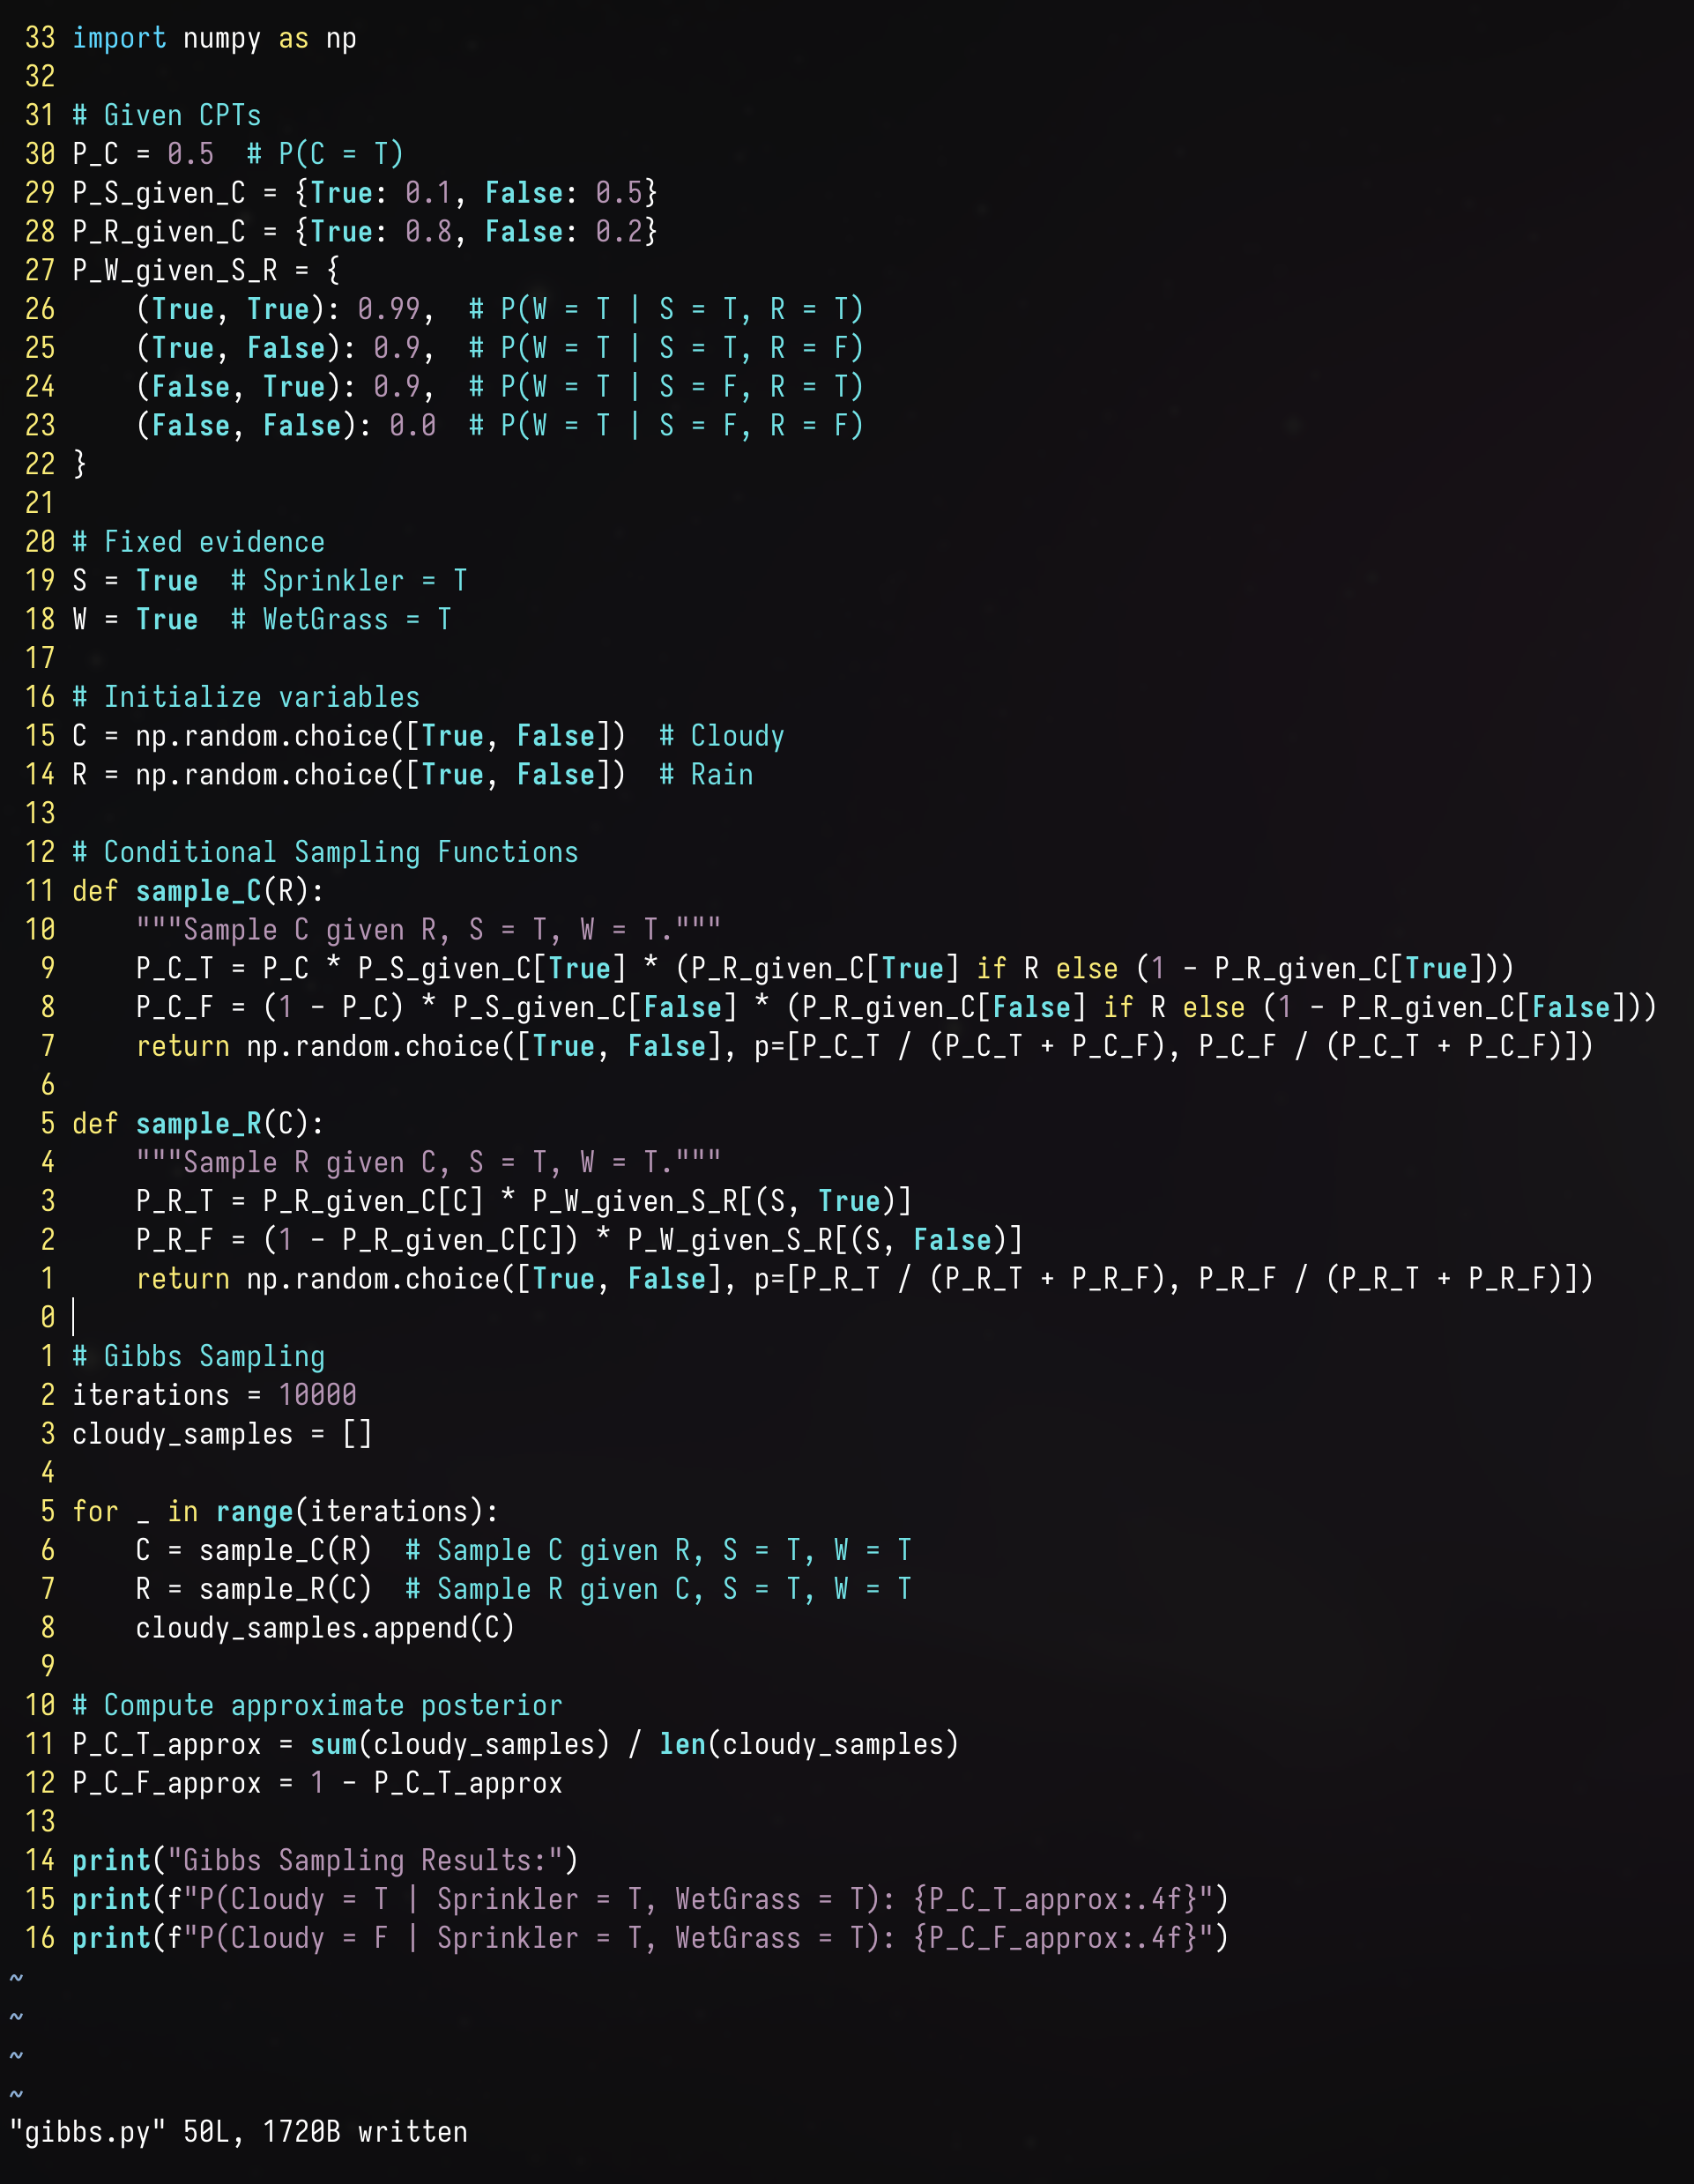
\includegraphics[width=0.8\textwidth]{ss.png}
    \caption{Gibbs Sampling Code Implementation}
\end{figure}

The resulting posterior probabilities are:

\[
P(\text{Cloudy} = T \mid \text{Sprinkler} = T, \text{WetGrass} = T) \approx 0.1778,
\]
\[
P(\text{Cloudy} = F \mid \text{Sprinkler} = T, \text{WetGrass} = T) \approx 0.8222.
\]

\section*{Problem 3: VAE Evidence Lower Bound (ELBO)}

Starting with the log marginal likelihood:

\[

\log p_\theta(x_i) = \log \sum_z p_\theta(x_i, z)
\]

Introduce the approximate posterior \( q_\phi(z | x_i) \) and multiply/divide by it:

\[
\log p_\theta(x_i) = \log \sum_z \frac{p_\theta(x_i, z) q_\phi(z | x_i)}{q_\phi(z | x_i)}.
\]

By Jensen's inequality (concavity of the logarithm):

\[
\log p_\theta(x_i) \geq \mathbb{E}_{q_\phi(z | x_i)} \left[ \log p_\theta(x_i, z) - \log q_\phi(z | x_i) \right].
\]

Expand the joint distribution \( p_\theta(x_i, z) = p_\theta(z) p_\theta(x_i | z) \):

\[
\log p_\theta(x_i) \geq \mathbb{E}_{q_\phi(z | x_i)} \left[ \log p_\theta(z) + \log p_\theta(x_i | z) - \log q_\phi(z | x_i) \right].
\]

Rearranging terms:

\[
\log p_\theta(x_i) \geq -D_{KL} \left( q_\phi(z | x_i) \| p_\theta(z) \right) + \mathbb{E}_{q_\phi(z | x_i)} \left[ \log p_\theta(x_i | z) \right].
\]

Thus, the ELBO (Evidence Lower Bound) is derived:

\[
\log p_\theta(x_i) \geq \mathcal{L} = -D_{KL} \left( q_\phi(z | x_i) \| p_\theta(z) \right) + \mathbb{E}_{q_\phi(z | x_i)} \left[ \log p_\theta(x_i | z) \right].
\]
---

\section*{Problem 4: RBM Movie Recommendation System}

\subsection*{4.1 Bipolar Coding Necessity}
Using $\pm 1$ instead of $0/1$ makes the Restricted Boltzmann Machine (RBM) more symmetric. When the visible and hidden units are centered around zero, the energy function and probability calculations become more balanced and mathematically cleaner. This symmetry can lead to simpler derivations and sometimes improved training stability.

\subsection*{4.2 Conditional Probability Formulation}
When switching from binary $\{0,1\}$ to bipolar $\{-1,+1\}$ coding, each $0$ is replaced with $-1$ and $1$ remains $+1$. To ensure that a zero-valued input corresponds to a 50\% probability for $+1$ and 50\% for $-1$, we rescale the input to the logistic (sigmoid) function by a factor of 2. Thus, for hidden units:
\[
P(h_j = +1 \mid v) = \sigma\bigl(2(W_{j,:}v + c_j)\bigr),
\]
and similarly for visible units:
\[
P(v_i = +1 \mid h) = \sigma\bigl(2(W_{i,:}h + b_i)\bigr),
\]
where $\sigma(x) = \frac{1}{1 + e^{-x}}$.

\subsection*{4.3 Predicting Preference for $\mathbf{m_2}$}
\textbf{Given:} The user liked $m_1$ ($m_1=+1$) and disliked $m_3$ ($m_3=-1$). We want to predict the preference for $m_2$.

\noindent\textbf{Steps:}
\begin{enumerate}
  \item \textbf{Known Visible Units:} Set $v = (m_1, m_2, m_3) = (+1,?, -1)$. We initially treat $m_2$ as unknown.
  
  \item \textbf{Hidden Input:} Compute $W^T v + c$. Given the parameters, this yields:
  \[
  W^T v + c = [-2,\,4,\,-2].
  \]

  \item \textbf{Hidden Probabilities:} For each hidden unit $h_j$:
  \[
  P(h_j=+1 \mid v) = \sigma(2(W_{j,:}v + c_j)) \implies h\_prob \approx [0.1192,\;0.9820,\;0.1192].
  \]

  \item \textbf{Hidden States:} Since $0.1192 < 0.5$ and $0.9820 > 0.5$:
  \[
  h_1 = -1, \quad h_2 = +1, \quad h_3 = -1.
  \]

  \item \textbf{Visible Reconstruction:} Using $h$, compute $W h + b$:
  \[
  W h + b = [1,\, -2,\, -6].
  \]
  
  Apply $\sigma$ (with factor 2 for bipolar):
  \[
  v\_prob = [\sigma(1), \sigma(-2), \sigma(-6)] \approx [0.7311,\;0.1192,\;0.0025].
  \]

  \item \textbf{Prediction for $m_2$:}
  \[
  P(m_2=+1) \approx 0.1192.
  \]
  Since $0.1192 < 0.5$, we predict:
  \[
  m_2 = -1 \quad (\text{user is predicted to dislike } m_2).
  \]
\end{enumerate}
\end{document}
